\section{proyectoRedes 1}\label{proyectoredes-1}

\subsection{Analisis Preliminar}\label{analisis-preliminar}

Distancias -aproximadas- entre las sedes de salud-Caracas:

\begin{longtable}[c]{@{}lllll@{}}
\toprule\addlinespace
& El Paraiso & San Antonio & Guarenas & Maiquetía
\\\addlinespace
\midrule\endhead
El Paraiso & & 25.8km & 40.7km & 28km
\\\addlinespace
San Antonio & 25.8km & & 57.7km & 47.8km
\\\addlinespace
Guarenas & 40.7km & 57.7km & & 65.4km
\\\addlinespace
Maiquetía & 28km & 47.8km & 65.4km &
\\\addlinespace
\bottomrule
\end{longtable}

De la tabla anterior, se puede apreciar que las dos sedes más distantes
son la de Maiquetía y la Guarenas, por lo que estas estarían conectadas
a través del ISP para ahorrar en lo posible los costos referentes a la
conexión física entre estas, tal y como indica el planteamiento del
problema.

Con el fin de mantener la carga de la red equilibrada, el analisis
lógico esperaría poder distribuir las sedes equitativamente entre ambos
ISP, sin embargo, dada la distancia física existente entre estas y el
costo que implica realizar una conexión física independiente al ISP, se
concluyó distribuir las sedes en dos grupos: El primer grupo conformado
por las sedes de El Paraiso, San Antonio y Maiquetía, y el segundo
conformado únicamente por la sede de Guarenas.

Una vez establecida la distribución general de la red, fue necesario
hacer el subneteo adecuado para diseñar la topología y posterior
configuració nde esta, así como el futuro calculo de los costos de los
implementes, entre otras decisiones asociadas a la implementación de la
red.

\subsection{Topología}\label{topologuxeda}

\subsubsection{Planteamiento de modelos}\label{planteamiento-de-modelos}

\paragraph{Modelo 1}\label{modelo-1}

\begin{figure}[htbp]
\centering
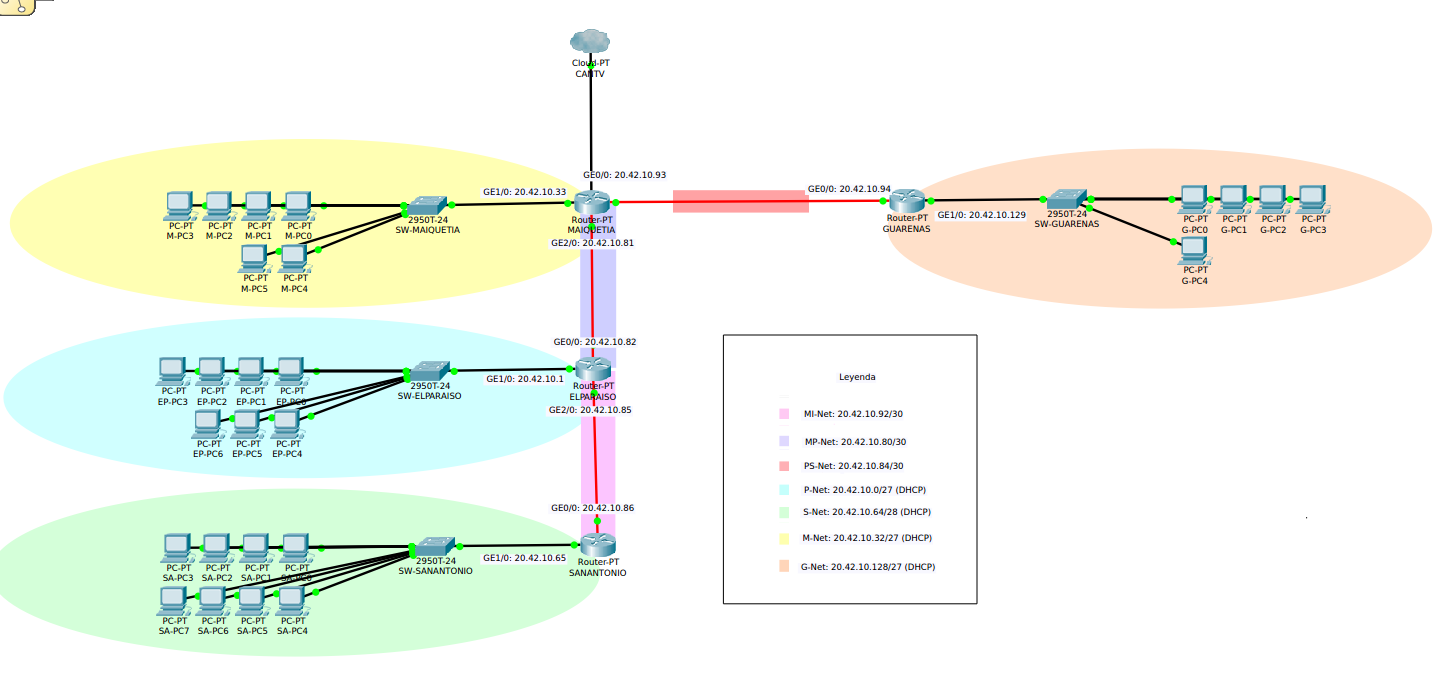
\includegraphics{ModeloAlternoCostosos.png}
\caption{Modelo alterno costoso}
\end{figure}

En este modelo, solo se conecta el enrutador de Maiquetía al ISP. Sin
embargo, los costos requeridos para interconectar Guatire-Maiquetía
tanto de cable de fibra óptica como trabajos de perforación y
mantenimiento, serían muy elevados, por lo que se descartó este modelo.

\paragraph{Modelo 2}\label{modelo-2}

En este modelo, las redes de Guarenas y Maiquetía estan conectadas
mediante el ISP, y Maiquetia establece conexión con El Paraiso y con San
Antonio. Este modelo fué descartado debido a los costos requeridos para
conectar Maiquetía y San Antonio, teniendo como alternativa inmediata el
próximo modelo.

\paragraph{Modelo 3}\label{modelo-3}

\begin{figure}[htbp]
\centering
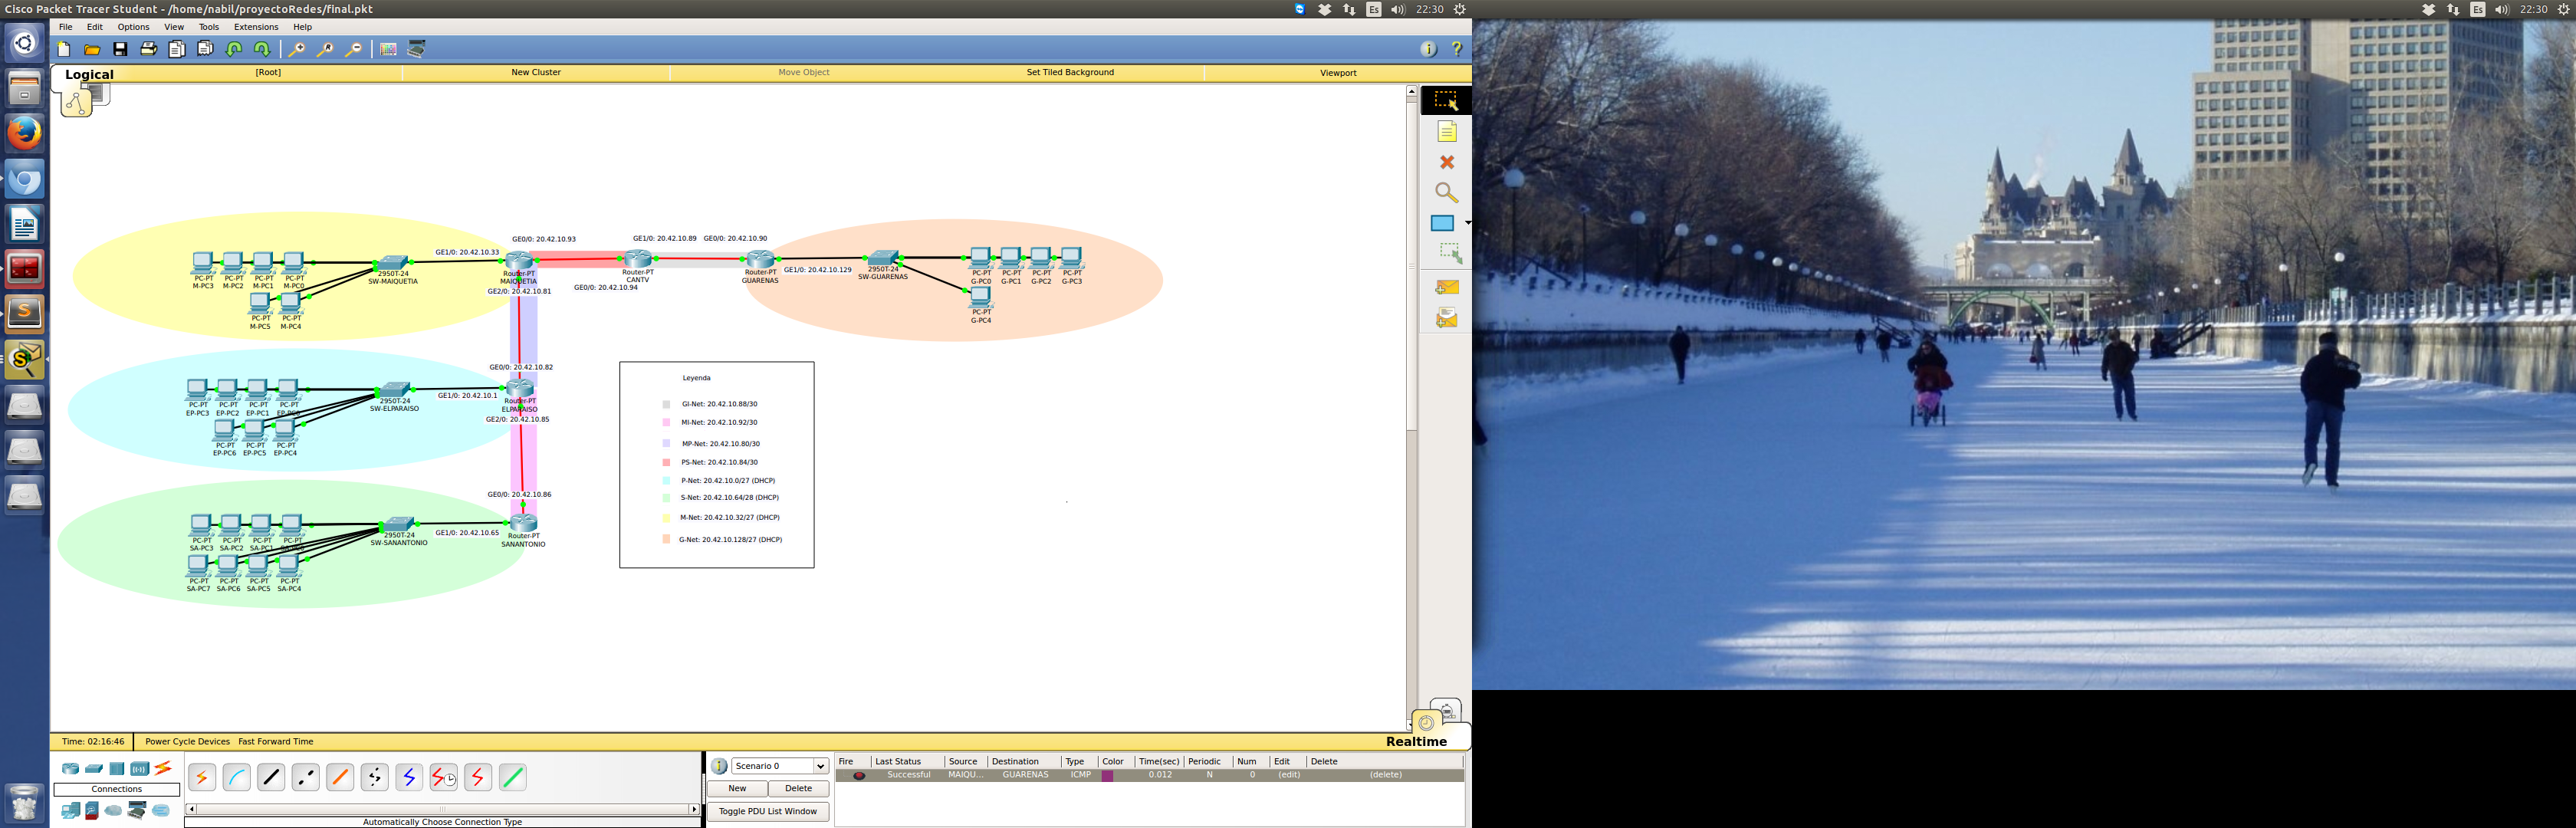
\includegraphics{ModeloFinal.jpg}
\caption{Modelo final}
\end{figure}

En este modelo, las redes de Guarenas y Maiquetía estan conectadas
mediante el ISP, y Maiquetia establece conexión con El Paraiso y este
con San Antonio. El enrutador de el paraiso funciona como enlace entre
Maiquetía y San Antonio. Este modelo fué el final a utilizar debido a su
buena gestión de recursos y eficiencia en la red. Sin embargo, para que
pudiese funcionar, fué requerido una defición de enrutamiento definida
más adelante.

\subsubsection{Descripción de la
topología}\label{descripciuxf3n-de-la-topologuxeda}

La topología escogida para implantar la red de salud-Caracas está basada
en la topología de tipo Árbol. Como nodo raiz, se tiene al enrutador de
CANTV, y los hijos inmediatos a estos son el enrutador de GUARENAS y el
enrutador de MAIQUETIA. En el siguiente nivel se encuentran el
conmutador de maiquetía, el enrutador de ELPARAISO y el conmutador de
Guarenas. Luego, se tienen a los hosts de Maiquetía, los host de
Guarenas, el conmutador de El Paraiso y el enrutador de SANANTONIO.
Luego de esto, están presente los host de El Paraiso y el conmutador de
San Antonio. En el último nivel, estan presentes los hosts de San
Antonio.

Para el caso particular de esta implantación, los ordenadores
representan las hojas del árbol ya que no tendrán hijos y los
conmutadores o los enrutadores representan el nodo padre de un árbol
subsiguiente.

\subsection{Esquema de
direccionamiento}\label{esquema-de-direccionamiento}

\subsubsection{Requisitos}\label{requisitos}

Tomando en cuenta que el crecimiento estimado se refiere a la cantidad
de host en la que puede incrementar la subred partiendo de la cantidad
presente, se tienen los siguientes requerimientos generales:

\begin{enumerate}
\def\labelenumi{\arabic{enumi}.}
\itemsep1pt\parskip0pt\parsep0pt
\item
  Una subred de 27 hosts para El paraiso (7 Actuales y 20 del
  crecimiento estimado).
\item
  Una subred de 8 hosts para San Antonio de los Altos.
\item
  Una subred de 15 hosts para Guarenas (5 Actuales y 10 del crecimiento
  estimado).
\item
  Una subred de 21 hosts para Maiquetía (6 Actuales y 15 del crecimiento
  estimado).
\end{enumerate}

\subsubsection{Analisís de requisitos:
Totalización.}\label{analisuxeds-de-requisitos-totalizaciuxf3n.}

En cuanto al direccionamiento IP se refiere, se decidió comprar el rango
de direcciones IP del ISP CANTV 20.42.10.0/24 debido a que se representa
a una clínica de alto alcance y se disponen los medios para ello. A su
vez, si se desea a futuro construir otra sede de salud-Caracas, se
dispondrían de direcciones IP para asignar a la nueva sede.

Estableciendo etiquetas para cada subred, se tiene:

P-net = El Paraiso. S-net = San Antonio de los Altos. G-net = Guarenas.
M-net = Maiquetía.

Inicialmente se poseen dos enrutadors con direcciones IP asignadas
mediante el ISP CANTV, cada uno con su respectiva subred.

\begin{longtable}[c]{@{}llll@{}}
\toprule\addlinespace
Subred & Nº Hosts & Crec. Estim. & enrutadors
\\\addlinespace
\midrule\endhead
P-net & 7 & 20 & 1
\\\addlinespace
M-net & 6 & 15 & 1
\\\addlinespace
G-net & 5 & 10 & 1
\\\addlinespace
S-net & 8 & 0 & 1
\\\addlinespace
\bottomrule
\end{longtable}

Sin embargo, al requerir interconectar los enrutadors de caracas (sin
utilizar costos adicionales en cables al tomar a El Paraiso como nodo
central), es necesario crear 2 sub-redes nuevas, MP-net y PS-net, a su
vez que son requeridas otras dos para las conexiones de Guarenas al ISP
y del ISP a Maiquetia. Actualizando la tabla anterior de esta manera:

\begin{longtable}[c]{@{}llll@{}}
\toprule\addlinespace
Subred & Nº Hosts & Crec. Estim. & enrutadors
\\\addlinespace
\midrule\endhead
P-net & 7 & 20 & 1
\\\addlinespace
M-net & 6 & 15 & 1
\\\addlinespace
G-net & 5 & 10 & 1
\\\addlinespace
S-net & 8 & 0 & 1
\\\addlinespace
MP-net & 2 & 0 & 0
\\\addlinespace
PS-net & 2 & 0 & 0
\\\addlinespace
GI-net & 2 & 0 & 0
\\\addlinespace
MI-net & 2 & 0 & 0
\\\addlinespace
\bottomrule
\end{longtable}

\begin{longtable}[c]{@{}llll@{}}
\toprule\addlinespace
\begin{minipage}[t]{0.17\columnwidth}\raggedright
TOTAL
\end{minipage} & \begin{minipage}[t]{0.17\columnwidth}\raggedright
34
\end{minipage} & \begin{minipage}[t]{0.17\columnwidth}\raggedright
45
\end{minipage} & \begin{minipage}[t]{0.17\columnwidth}\raggedright
4
\end{minipage}
\\\addlinespace
\bottomrule
\end{longtable}

A partir de la tabla anterior, se puede inferir la cantidad de host
necesarios para cada supra-red principal, siendo:

\emph{PMS-net = P-net, S-net, M-net, MP-net y PS-net. }G-net = G-net.

\begin{longtable}[c]{@{}lllllll@{}}
\toprule\addlinespace
Subred & Nº Hosts & Crec. Estim. & enrutadors & Total Req. & Máscara &
IP's Libres
\\\addlinespace
\midrule\endhead
PMS-net & 25 & 35 & 3 & 63 & /25 & 63
\\\addlinespace
G-net & 5 & 10 & 1 & 16 & /27 & 14
\\\addlinespace
\bottomrule
\end{longtable}

A pesar de que para la G-net se estan desperdiciando 14 direcciones,
utilizar una máscara más pequeña implicaría aumentar los costos al tener
que utilizar otro enrutador con máscara de /30 y los otros instrumentos
asociados (Conmutadores, cables, interfaces de red). Como se esta
considerando la mejor opción costo-rendimiento, se dejarán libres esa
cantidad de direcciones con el fin de evitar costos adicionales.
Análogamente para la PMS-net.

\subsubsection{Analisís de requisitos: Información detallada de las
subredes.}\label{analisuxeds-de-requisitos-informaciuxf3n-detallada-de-las-subredes.}

Sin procesar las subredes en PMS-net, se tiene:

Luego se aplicó la técnica de LVSM para distribución de direcciones IP
en estas subredes, debido a que existen diferencias notables en cuanto a
la cantidad de hosts requeridas por cada subred como para realizar una
distribución estática. Luego de aplicar esta técnica, se obtuvo:

\begin{longtable}[c]{@{}llllll@{}}
\toprule\addlinespace
Subred & Máscara & Dir Subred & Broadcast & Rango & D. Libres
\\\addlinespace
\midrule\endhead
PMS-net & 255.255.255.128 & 20.42.10.0 & 20.42.10.127 & .1 - .126 & 63
\\\addlinespace
G-net & 255.255.255.224 & 20.42.10.128 & 20.42.10.159 & .129 - .159 & 14
\\\addlinespace
\bottomrule
\end{longtable}

Y las subredes de PMS-net estan conformadas de esta manera:

\begin{longtable}[c]{@{}llllll@{}}
\toprule\addlinespace
Subred & Máscara & Dir Subred & Broadcast & Rango & D. Libres
\\\addlinespace
\midrule\endhead
P-net & 255.255.255.224 & 20.42.10.0 & 20.42.10.31 & .1 - .30 & 2
\\\addlinespace
M-net & 255.255.255.224 & 20.42.10.32 & 20.42.10.63 & .33 - .62 & 8
\\\addlinespace
S-net & 255.255.255.240 & 20.42.10.64 & 20.42.10.79 & .65 - .78 & 5
\\\addlinespace
MP-net & 255.255.255.252 & 20.42.10.80 & 20.42.10.83 & .81 - .82 & 0
\\\addlinespace
PS-net & 255.255.255.252 & 20.42.10.84 & 20.42.10.87 & .85 - .86 & 0
\\\addlinespace
GI-net & 255.255.255.252 & 20.42.10.88 & 20.42.10.91 & .89 - .90 & 0
\\\addlinespace
MI-net & 255.255.255.252 & 20.42.10.92 & 20.42.10.95 & .93 - .94 & 0
\\\addlinespace
\bottomrule
\end{longtable}

\subsection{Enrutamiento}\label{enrutamiento}

\subsubsection{Descripción del
enrutamiento}\label{descripciuxf3n-del-enrutamiento}

Debido a la topología escogida, es necesario definir un enrutamiento
adecuado para poder interconectar adecuadamente las subredes entre sí y
que estas conozcan a que enrutador siguiente consultar.

A pesar de disponer de la opción de utilizar enrutamiento dinámico, se
decidió utilizar enrutamiento estático ya que la carga extra que
requiere el enrutamiento dinámico es innecesaria para la topología
escogida. Así, cada enrutador se encarga o bien de enviar el paquete a
un host de su subred o de enviarlo al siguiente enrutador que contenga
la tabla de enrutamiento de la subred a la que va dirigida el paquete
recibido o conozca a que enrutador reenviarlo.

\subsubsection{Código implantado}\label{cuxf3digo-implantado}

Se utilizó el Control Line Interface de cada enrutador para configurar
el enrutamiento estático correspondiente.

\begin{verbatim}
SANANTONIO(config)#ip route 20.42.10.0 255.255.255.224 20.42.10.85
SANANTONIO(config)#ip route 20.42.10.32 255.255.255.224 20.42.10.85
SANANTONIO(config)#ip route 20.42.10.80 255.255.255.252 20.42.10.85
SANANTONIO(config)#ip route 20.42.10.92 255.255.255.252 20.42.10.85
SANANTONIO(config)#ip route 20.42.10.128 255.255.255.224 20.42.10.85
SANANTONIO(config)#ip route 20.42.10.88 255.255.255.252 20.42.10.85

---------------------------

ELPARAISO(config)#ip route 20.42.10.32 255.255.255.224 20.42.10.81
ELPARAISO(config)#ip route 20.42.10.88 255.255.255.252 20.42.10.81
ELPARAISO(config)#ip route 20.42.10.92 255.255.255.252 20.42.10.81
ELPARAISO(config)#ip route 20.42.10.128 255.255.255.224 20.42.10.81
ELPARAISO(config)#ip route 20.42.10.64 255.255.255.240 20.42.10.86

---------------------------

MAIQUETIA(config)#ip route 20.42.10.0 255.255.255.224 20.42.10.82
MAIQUETIA(config)#ip route 20.42.10.64 255.255.255.240 20.42.10.82
MAIQUETIA(config)#ip route 20.42.10.84 255.255.255.252 20.42.10.82
MAIQUETIA(config)#ip route 20.42.10.88 255.255.255.252 20.42.10.94
MAIQUETIA(config)#ip route 20.42.10.128 255.255.255.224 20.42.10.94

--------------------------

CANTV(config)#ip route 20.42.10.0 255.255.255.224 20.42.10.93
CANTV(config)#ip route 20.42.10.32 255.255.255.224 20.42.10.93
CANTV(config)#ip route 20.42.10.64 255.255.255.224 20.42.10.93
CANTV(config)#ip route 20.42.10.64 255.255.255.240 20.42.10.93
CANTV(config)#ip route 20.42.10.80 255.255.255.252 20.42.10.93
CANTV(config)#ip route 20.42.10.84 255.255.255.252 20.42.10.93


--------------------------

GUARENAS(config)#ip route 20.42.10.0 255.255.255.224 20.42.10.89
GUARENAS(config)#ip route 20.42.10.32 255.255.255.224 20.42.10.89
GUARENAS(config)#ip route 20.42.10.64 255.255.255.240 20.42.10.89
GUARENAS(config)#ip route 20.42.10.80 255.255.255.252 20.42.10.89
GUARENAS(config)#ip route 20.42.10.84 255.255.255.252 20.42.10.89
GUARENAS(config)#ip route 20.42.10.92 255.255.255.252 20.42.10.89
\end{verbatim}

\subsection{Direccionamiento IP}\label{direccionamiento-ip}

\subsubsection{Descripción del direccionamiento
IP}\label{descripciuxf3n-del-direccionamiento-ip}

DHCP pq crecimiento y bajones de luz como emergencia and stuff

Se utilizó DHCP ya que esto facilita la configuración en presencia de
subredes grandes o que poseen un crecimiento estimado considerable.
Adicionalmente a lo anterior, en ninguna de las subredes diseñadas para
salud-Caracas se ofrecen servicios fuera de los routers, por lo que no
era necesario establecer direcciones estáticas en estas. Además,
representa un ahorro en la configuración de la red en la que se disponga
de este servidor DHCP en el momento en el que se adquieran nuevos
ordenadores y se conecten a la red: ni estos, ni el servidor, requerian
alguna configuración adicional a la proporcionada por defecto.

\subsubsection{Código implantado}\label{cuxf3digo-implantado-1}

Se utilizó el Control Line Interface de cada enrutador para configurar
el servidor DHCP asociado a la subred que cada enrutador esté encargado
de interconectar.

\begin{verbatim}
GUARENAS(config)#ip dhcp pool GNET
GUARENAS(dhcp-config)#network 20.42.10.128 255.255.255.224
GUARENAS(dhcp-config)#default-enrutador 20.42.10.129
GUARENAS(dhcp-config)#dns-server 8.8.8.8
GUARENAS(dhcp-config)#exit
GUARENAS(config)#dowr

---------------------------

MAIQUETIA(config-if)#ip dhcp pool MNET
MAIQUETIA(dhcp-config)#network 20.42.10.32 255.255.255.224
MAIQUETIA(dhcp-config)#default-enrutador 20.42.10.33
MAIQUETIA(dhcp-config)#dns-server 8.8.8.8
MAIQUETIA(dhcp-config)#exit
MAIQUETIA(config)#do wr

---------------------------

ELPARAISO(config-if)#ip dhcp pool PNET
ELPARAISO(dhcp-config)#network 20.42.10.0 255.255.255.224
ELPARAISO(dhcp-config)#dns-server 8.8.8.8
ELPARAISO(dhcp-config)#default-enrutador 20.42.10.1
ELPARAISO(dhcp-config)#exit
ELPARAISO(config)#do wr

---------------------------

SANANTONIO(config-if)#ip dhcp pool SNET
SANANTONIO(dhcp-config)#default-enrutador 20.42.10.65
SANANTONIO(dhcp-config)#dns-server 8.8.8.8
SANANTONIO(dhcp-config)#network 20.42.10.64 255.255.255.240
SANANTONIO(dhcp-config)#exit
SANANTONIO(config)#do wr
\end{verbatim}

\subsection{Dispositivos requeridos}\label{dispositivos-requeridos}

\subsubsection{Requerimientos mínimos}\label{requerimientos-muxednimos}

\subsubsection{Costos}\label{costos}

Switch Tp-link 24 Puertos 10/100mbps Tl-sf1024 Rackeable Bs. 104.85000

de swiches and stuff
